    Vivamus congue volutpat elit non semper. Praesent molestie nec erat ac
    interdum. In quis suscipit erat. \textbf{Phasellus mauris felis, molestie
    ac pharetra quis}, tempus nec ante. Donec finibus ante vel purus mollis
    fermentum. Sed felis mi, pharetra eget nibh a, feugiat eleifend dolor. Nam
    mollis condimentum purus quis sodales. Nullam eu felis eu nulla eleifend
    bibendum nec eu lorem. Vivamus felis velit, volutpat ut facilisis ac,
    commodo in metus.


\newsavebox{\looseIRlisting}
\begin{lrbox}{\looseIRlisting}% Store first listing
\minipage{.68\textwidth}
\begin{lstlisting}
define VOID @kernel (%in0, %in1) (%out0, %out1):
	%tmp1 = %in0
	%tmp2 = %tmp1 * %tmp1 * %tmp1
	%tmp3 = %in1
	%tmp4 = %tmp2 + %tmp3
	%tmp5 = %tmp4
	%tmp6 = %tmp2 - %tmp3
	%tmp7 = %tmp6
	%out0 = %tmp5
	%out1 = %tmp7
\end{lstlisting}
\endminipage
\end{lrbox}

\newsavebox{\tightIRlisting}
\begin{lrbox}{\tightIRlisting}% Store first listing
\minipage{.68\textwidth}
\begin{lstlisting}
define VOID @kernel (new #list(in), new #list(out)):
	new #tmp2 = #in[0] * #in[0] * #in[0]
	#out[0] = #tmp2 + #in[1]
	#out[1] = #tmp2 - #in[1]
	<return nothing>
\end{lstlisting}
\endminipage
\end{lrbox}

\begin{figure}
\centering

\sbox{\measurebox}{%
  \begin{minipage}{.68\textwidth} \centering
        \subfloat[Loose IR]{\label{fig:figB}\usebox{\looseIRlisting}}
        \vspace{1em}
        \subfloat[Tight IR]{\label{fig:figC}\usebox{\tightIRlisting}}
  \end{minipage}
}

\usebox{\measurebox}\qquad
    \begin{minipage}[][\ht\measurebox][c]{.26\textwidth}
      \subfloat[Input DAG]{\label{fig:loose_tight_dag}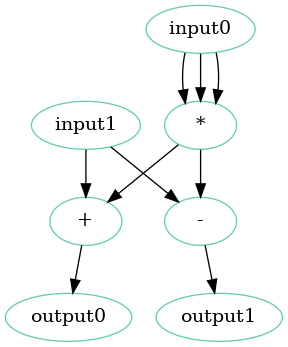
\includegraphics[width=\textwidth]{tight_vs_loose.png}}
       
    \end{minipage}
\caption{Example of the difference between a loose IR and tight IR. Figure \ref{fig:loose_tight_dag} shows the corresponding input DAG.} 
\label{fig:tight_loose}
\end{figure}

    \begin{figure}[h!]
    \begin{center}
        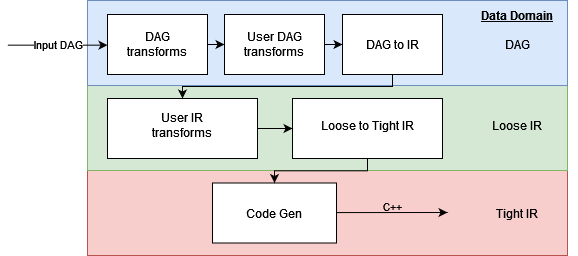
\includegraphics[width=.7
        \textwidth]{comp-arch.png}
        \caption{Overview of FLAT's architecture.}
        \label{fig:arch}
    \end{center}
\end{figure}